\chapter{グラフの基礎知識 - Basics of graphs}

競技プログラミング問題のいくつかは、問題をグラフの問題としてモデル化して適切なアルゴリズムを用いることで解決することができます。
グラフの典型的な例として、街を道路でつなぐネットワークとみなして最短の経路を求める問題などあります。
しかし、コンテストではグラフが問題の中に隠れていてグラフを用いるという発見が難しいことも多々あります。

このパートでは、特に競技プログラミングで重要となるトピックを中心に解説します。
この章では、グラフに関する概念を述べ、実装で必要になるグラフのさまざまな表現方法について述べます。

\section{グラフの用語 - Graph terminolog}

\index{Graph}
\index{node}
\index{edge}

\key{グラフ - graph}は\key{ノード - node}と\key{辺 - edge}から構成されます。
本書では以降、変数$n$はグラフのノード数、変数$m$は辺の数を表します。
ノードには$1,2,v \ldots ,n$の整数を用いて表します(訳註: 0-indexedではありません)。

例えば、次のグラフは5つのノードと7つのエッジから構成されています。

\begin{center}
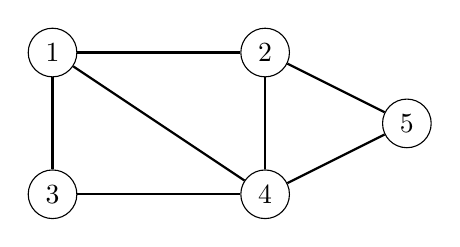
\begin{tikzpicture}[scale=0.9]
\node[draw, circle] (1) at (1,3) {$1$};
\node[draw, circle] (2) at (4,3) {$2$};
\node[draw, circle] (3) at (1,1) {$3$};
\node[draw, circle] (4) at (4,1) {$4$};
\node[draw, circle] (5) at (6,2) {$5$};

\path[draw,thick,-] (1) -- (2);
\path[draw,thick,-] (1) -- (3);
\path[draw,thick,-] (1) -- (4);
\path[draw,thick,-] (3) -- (4);
\path[draw,thick,-] (2) -- (4);
\path[draw,thick,-] (2) -- (5);
\path[draw,thick,-] (4) -- (5);
\end{tikzpicture}
\end{center}

\index{path}

ノード$a$からノード$b$まで、グラフの辺を通る経路(パス - path)があります。
パスの長さは、その中に含まれる辺の数とします。
例えば、上のグラフにはノード1からノード5まで長さ3のパス
 $1 \rightarrow 3 \rightarrow 4 \rightarrow 5$
 が存在します。

\begin{center}
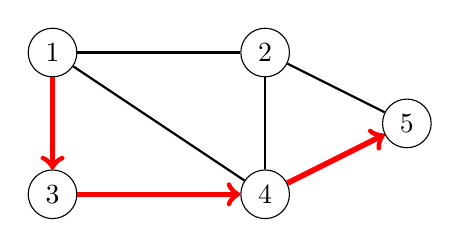
\begin{tikzpicture}[scale=0.9]
\node[draw, circle] (1) at (1,3) {$1$};
\node[draw, circle] (2) at (4,3) {$2$};
\node[draw, circle] (3) at (1,1) {$3$};
\node[draw, circle] (4) at (4,1) {$4$};
\node[draw, circle] (5) at (6,2) {$5$};

\path[draw,thick,-] (1) -- (2);
\path[draw,thick,-] (1) -- (3);
\path[draw,thick,-] (1) -- (4);
\path[draw,thick,-] (3) -- (4);
\path[draw,thick,-] (2) -- (4);
\path[draw,thick,-] (2) -- (5);
\path[draw,thick,-] (4) -- (5);

\path[draw=red,thick,->,line width=2pt] (1) -- (3);
\path[draw=red,thick,->,line width=2pt] (3) -- (4);
\path[draw=red,thick,->,line width=2pt] (4) -- (5);
\end{tikzpicture}
\end{center}

\index{cycle}

最初と最後のノードが同じものは\texttt{閉路(サイクル, Cycle)}と呼ばれます。
例えば、 上のグラフは
$1 \rightarrow 3 \rightarrow 4 \rightarrow 1$.
という閉路を含みます。

各ノードの出現回数が せいぜい1回であるパスは\texttt{単純}と呼ばれます。

%
% \begin{itemize}
% \item $1 \rightarrow 2 \rightarrow 5$ (length 2)
% \item $1 \rightarrow 4 \rightarrow 5$ (length 2)
% \item $1 \rightarrow 2 \rightarrow 4 \rightarrow 5$ (length 3)
% \item $1 \rightarrow 3 \rightarrow 4 \rightarrow 5$ (length 3)
% \item $1 \rightarrow 4 \rightarrow 2 \rightarrow 5$ (length 3)
% \item $1 \rightarrow 3 \rightarrow 4 \rightarrow 2 \rightarrow 5$ (length 4)
% \end{itemize}

\subsubsection{連結 - Connectivity}

\index{connected graph}

グラフは、ある任意の2つのノード間にパスが存在する場合、\key{連結}といいます。
例えば 、次のようなグラフは連結と呼ばれます。

\begin{center}
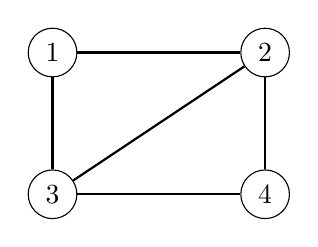
\begin{tikzpicture}[scale=0.9]
\node[draw, circle] (1) at (1,3) {$1$};
\node[draw, circle] (2) at (4,3) {$2$};
\node[draw, circle] (3) at (1,1) {$3$};
\node[draw, circle] (4) at (4,1) {$4$};
\path[draw,thick,-] (1) -- (2);
\path[draw,thick,-] (1) -- (3);
\path[draw,thick,-] (2) -- (3);
\path[draw,thick,-] (3) -- (4);
\path[draw,thick,-] (2) -- (4);
\end{tikzpicture}
\end{center}

次のグラフは、ノード4から他のノードに行くことができないので、
連結ではないグラフです(非連結)。

\begin{center}
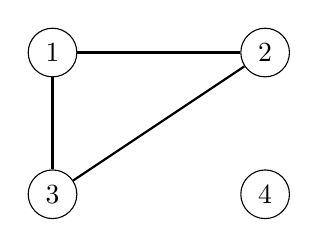
\begin{tikzpicture}[scale=0.9]
\node[draw, circle] (1) at (1,3) {$1$};
\node[draw, circle] (2) at (4,3) {$2$};
\node[draw, circle] (3) at (1,1) {$3$};
\node[draw, circle] (4) at (4,1) {$4$};
\path[draw,thick,-] (1) -- (2);
\path[draw,thick,-] (1) -- (3);
\path[draw,thick,-] (2) -- (3);
\end{tikzpicture}
\end{center}

\index{component}

グラフの各連結な部分を\key{成分(components)}を成分と呼びます。
例えば、次のグラフは3つの成分を含
んでいます。
$\{1,\,2,\,3\}$,
$\{4,\,5,\,6,\,7\}$,
$\{8\}$です。

\begin{center}
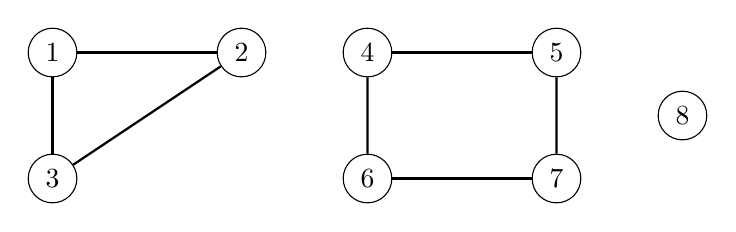
\begin{tikzpicture}[scale=0.8]
\node[draw, circle] (1) at (1,3) {$1$};
\node[draw, circle] (2) at (4,3) {$2$};
\node[draw, circle] (3) at (1,1) {$3$};

\node[draw, circle] (6) at (6,1) {$6$};
\node[draw, circle] (7) at (9,1) {$7$};
\node[draw, circle] (4) at (6,3) {$4$};
\node[draw, circle] (5) at (9,3) {$5$};

\node[draw, circle] (8) at (11,2) {$8$};

\path[draw,thick,-] (1) -- (2);
\path[draw,thick,-] (2) -- (3);
\path[draw,thick,-] (1) -- (3);
\path[draw,thick,-] (4) -- (5);
\path[draw,thick,-] (5) -- (7);
\path[draw,thick,-] (6) -- (7);
\path[draw,thick,-] (6) -- (4);
\end{tikzpicture}
\end{center}

\index{tree}

\key{木(tree})は、$n$個のノードと$n - 1$個の辺からなる連結グラフのことです。
木の任意の2つのノード間にはちょうど一本のパスが存在します。
例えば、次のグラフは木である。

\begin{center}
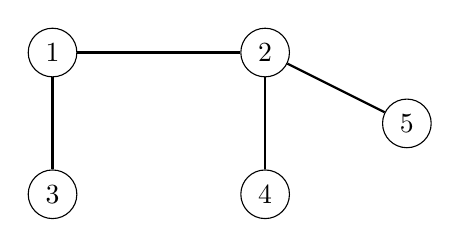
\begin{tikzpicture}[scale=0.9]
\node[draw, circle] (1) at (1,3) {$1$};
\node[draw, circle] (2) at (4,3) {$2$};
\node[draw, circle] (3) at (1,1) {$3$};
\node[draw, circle] (4) at (4,1) {$4$};
\node[draw, circle] (5) at (6,2) {$5$};

\path[draw,thick,-] (1) -- (2);
\path[draw,thick,-] (1) -- (3);
%\path[draw,thick,-] (1) -- (4);
\path[draw,thick,-] (2) -- (5);
\path[draw,thick,-] (2) -- (4);
%\path[draw,thick,-] (4) -- (5);
\end{tikzpicture}
\end{center}

\subsubsection{有向と無向 - Edge directions}

\index{directed graph}

グラフの辺が決まった方向にしか移動できない場合、\key{有向(directed)}と呼ばれます。
例えば、次のようなグラフは有向です。

\begin{center}
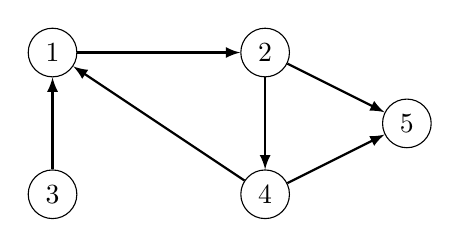
\begin{tikzpicture}[scale=0.9]
\node[draw, circle] (1) at (1,3) {$1$};
\node[draw, circle] (2) at (4,3) {$2$};
\node[draw, circle] (3) at (1,1) {$3$};
\node[draw, circle] (4) at (4,1) {$4$};
\node[draw, circle] (5) at (6,2) {$5$};
\path[draw,thick,->,>=latex] (1) -- (2);
\path[draw,thick,->,>=latex] (2) -- (4);
\path[draw,thick,->,>=latex] (2) -- (5);
\path[draw,thick,->,>=latex] (4) -- (5);
\path[draw,thick,->,>=latex] (4) -- (1);
\path[draw,thick,->,>=latex] (3) -- (1);
\end{tikzpicture}
\end{center}

このグラフには、ノード3からノード5へのパス
$3 \rightarrow 1 \rightarrow 2 \rightarrow 5$
がありますが、
ノード5からノード3へのパスは存在しません。

\subsubsection{辺の重み - Edge weights}

\index{weighted graph}

\key{重み付きグラフ}では、各辺に\key{重み}が割り当てられています。
重みは辺の長さのようなものです。
重み付きグラフの例を次に示します。

\begin{center}
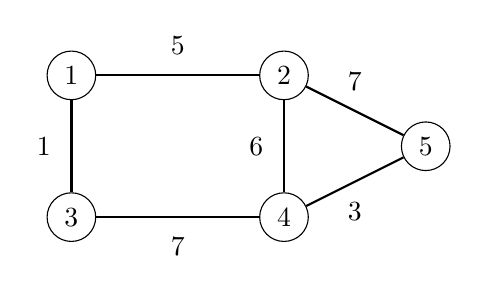
\begin{tikzpicture}[scale=0.9]
\node[draw, circle] (1) at (1,3) {$1$};
\node[draw, circle] (2) at (4,3) {$2$};
\node[draw, circle] (3) at (1,1) {$3$};
\node[draw, circle] (4) at (4,1) {$4$};
\node[draw, circle] (5) at (6,2) {$5$};
\path[draw,thick,-] (1) -- node[font=\small,label=above:5] {} (2);
\path[draw,thick,-] (1) -- node[font=\small,label=left:1] {} (3);
\path[draw,thick,-] (3) -- node[font=\small,label=below:7] {} (4);
\path[draw,thick,-] (2) -- node[font=\small,label=left:6] {} (4);
\path[draw,thick,-] (2) -- node[font=\small,label=above:7] {} (5);
\path[draw,thick,-] (4) -- node[font=\small,label=below:3] {} (5);
\end{tikzpicture}
\end{center}

重み付きグラフのパスの長さは、パス上の辺の重みの和で表します。
例えば、上のグラフでは、$1 \rightarrow 2 \rightarrow 5$ のパスの長さは$12$。
$1 \rightarrow 3 \rightarrow 4 \rightarrow 5$のパスの長さは$11$です。
後者の経路はこのグラフのノード1からノード5への\key{最短経路}です。

\subsubsection{隣接ノードと次数 - Neighbors and degrees}

\index{neighbor}
\index{degree}


2つのノードは、その間にエッジがある場合、\key{隣接(neighbors, adjacent)}であるといいます。
\key{次数(degree)}は、ノードの隣接するノードの数です。
例えば、次のグラフでは、ノード2の近傍は1、4、5なので、その次数は3です。

\begin{center}
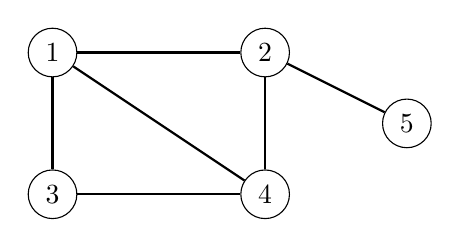
\begin{tikzpicture}[scale=0.9]
\node[draw, circle] (1) at (1,3) {$1$};
\node[draw, circle] (2) at (4,3) {$2$};
\node[draw, circle] (3) at (1,1) {$3$};
\node[draw, circle] (4) at (4,1) {$4$};
\node[draw, circle] (5) at (6,2) {$5$};

\path[draw,thick,-] (1) -- (2);
\path[draw,thick,-] (1) -- (3);
\path[draw,thick,-] (1) -- (4);
\path[draw,thick,-] (3) -- (4);
\path[draw,thick,-] (2) -- (4);
\path[draw,thick,-] (2) -- (5);
%\path[draw,thick,-] (4) -- (5);
\end{tikzpicture}
\end{center}

グラフに含まれる頂点の次数の和は常に$2m$($m$は辺の数)となります。
なぜなら、各辺はちょうど2つのノードの度数を1つずつ増加させるからです。
このため、次数の和は常に偶数となります。

\index{regular graph}
\index{complete graph}

グラフは、すべてのノードの次数が同じ(例えば定数$d$)であれば\key{正則(regular)}グラフです。
すべてのノードの次数が$n - 1$であれば、すなわちグラフがノード間の可能なすべての辺を含んでいれば、
\key{完全(complete)}グラフです。

\index{indegree}
\index{outdegree}


有向グラフでにおいて各頂点には入次数と出次数があります。
\key{入次数(indegree)}とはそのノードで終わる辺の数、
\key{出次数(outdegree)}そのノードで始まる辺の数です。
例えば、次のグラフでは、ノード2の入次数は2、ノード2の出次数は1です。

\begin{center}
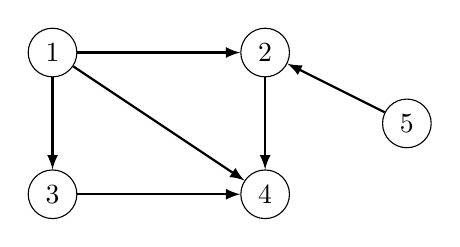
\begin{tikzpicture}[scale=0.9]
\node[draw, circle] (1) at (1,3) {$1$};
\node[draw, circle] (2) at (4,3) {$2$};
\node[draw, circle] (3) at (1,1) {$3$};
\node[draw, circle] (4) at (4,1) {$4$};
\node[draw, circle] (5) at (6,2) {$5$};

\path[draw,thick,->,>=latex] (1) -- (2);
\path[draw,thick,->,>=latex] (1) -- (3);
\path[draw,thick,->,>=latex] (1) -- (4);
\path[draw,thick,->,>=latex] (3) -- (4);
\path[draw,thick,->,>=latex] (2) -- (4);
\path[draw,thick,<-,>=latex] (2) -- (5);
\end{tikzpicture}
\end{center}

\subsubsection{グラフの着色 - Colorings}

\index{coloring}
\index{bipartite graph}

グラフの\key{色付け(coloring)}は、隣接するノードが同じ色にならないように、各ノードに色を割り当てることをいいます。
グラフを2色で色付けできる場合、\key{二部グラフ(bipartite graph)} であるといいます。
なお、二部グラフである条件として奇数本の辺で構成される閉路が存在しないグラフに限られることが分かっています。

例を示します。

\begin{center}
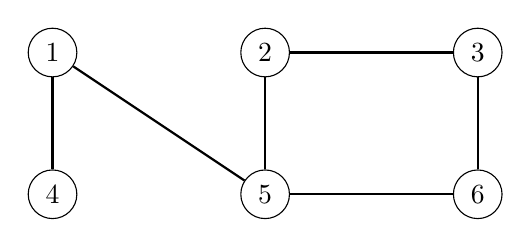
\begin{tikzpicture}[scale=0.9]
\node[draw, circle] (1) at (1,3) {$2$};
\node[draw, circle] (2) at (4,3) {$3$};
\node[draw, circle] (3) at (1,1) {$5$};
\node[draw, circle] (4) at (4,1) {$6$};
\node[draw, circle] (5) at (-2,1) {$4$};
\node[draw, circle] (6) at (-2,3) {$1$};
\path[draw,thick,-] (1) -- (2);
\path[draw,thick,-] (1) -- (3);
\path[draw,thick,-] (3) -- (4);
\path[draw,thick,-] (2) -- (4);
\path[draw,thick,-] (3) -- (6);
\path[draw,thick,-] (5) -- (6);
\end{tikzpicture}
\end{center}
このグラフは次のように着色でき、二部グラフです。
\begin{center}
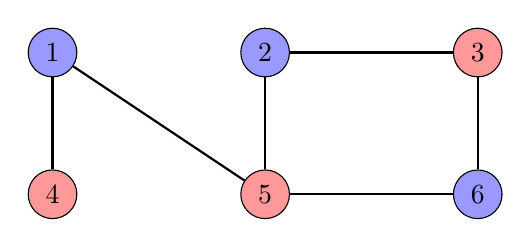
\begin{tikzpicture}[scale=0.9]
\node[draw, circle, fill=blue!40] (1) at (1,3) {$2$};
\node[draw, circle, fill=red!40] (2) at (4,3) {$3$};
\node[draw, circle, fill=red!40] (3) at (1,1) {$5$};
\node[draw, circle, fill=blue!40] (4) at (4,1) {$6$};
\node[draw, circle, fill=red!40] (5) at (-2,1) {$4$};
\node[draw, circle, fill=blue!40] (6) at (-2,3) {$1$};
\path[draw,thick,-] (1) -- (2);
\path[draw,thick,-] (1) -- (3);
\path[draw,thick,-] (3) -- (4);
\path[draw,thick,-] (2) -- (4);
\path[draw,thick,-] (3) -- (6);
\path[draw,thick,-] (5) -- (6);
\end{tikzpicture}
\end{center}
次のグラフはどうでしょうか?
\begin{center}
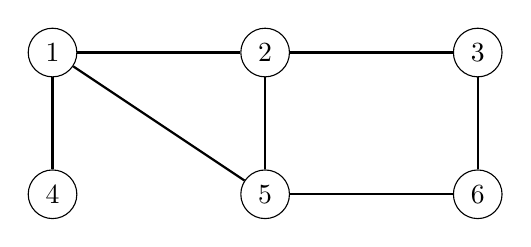
\begin{tikzpicture}[scale=0.9]
\node[draw, circle] (1) at (1,3) {$2$};
\node[draw, circle] (2) at (4,3) {$3$};
\node[draw, circle] (3) at (1,1) {$5$};
\node[draw, circle] (4) at (4,1) {$6$};
\node[draw, circle] (5) at (-2,1) {$4$};
\node[draw, circle] (6) at (-2,3) {$1$};
\path[draw,thick,-] (1) -- (2);
\path[draw,thick,-] (1) -- (3);
\path[draw,thick,-] (3) -- (4);
\path[draw,thick,-] (2) -- (4);
\path[draw,thick,-] (3) -- (6);
\path[draw,thick,-] (5) -- (6);
\path[draw,thick,-] (1) -- (6);
\end{tikzpicture}
\end{center}
は2分割ではありません。なぜなら、以下の閉路を2色で色塗りできないためです。
\begin{center}
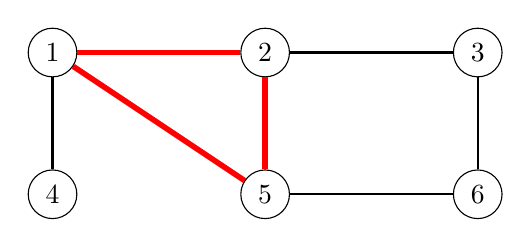
\begin{tikzpicture}[scale=0.9]
\node[draw, circle] (1) at (1,3) {$2$};
\node[draw, circle] (2) at (4,3) {$3$};
\node[draw, circle] (3) at (1,1) {$5$};
\node[draw, circle] (4) at (4,1) {$6$};
\node[draw, circle] (5) at (-2,1) {$4$};
\node[draw, circle] (6) at (-2,3) {$1$};
\path[draw,thick,-] (1) -- (2);
\path[draw,thick,-] (1) -- (3);
\path[draw,thick,-] (3) -- (4);
\path[draw,thick,-] (2) -- (4);
\path[draw,thick,-] (3) -- (6);
\path[draw,thick,-] (5) -- (6);
\path[draw,thick,-] (1) -- (6);

\path[draw=red,thick,-,line width=2pt] (1) -- (3);
\path[draw=red,thick,-,line width=2pt] (3) -- (6);
\path[draw=red,thick,-,line width=2pt] (6) -- (1);
\end{tikzpicture}
\end{center}

\subsubsection{単純グラフ - Simplicity}

\index{simple graph}

始点と終点が同じノードの辺がなく、
ある2つのノード間に複数の辺が存在しない場合、グラフは\key{単純グラフ(simple graph)}と呼ばれます。
大半の場合、グラフは単純でと仮定されます。
例えば、次のようなグラフは単純ではありません。

\begin{center}
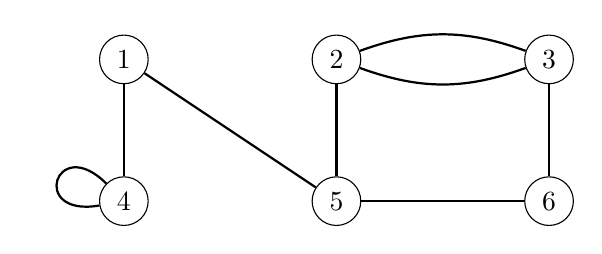
\begin{tikzpicture}[scale=0.9]
\node[draw, circle] (1) at (1,3) {$2$};
\node[draw, circle] (2) at (4,3) {$3$};
\node[draw, circle] (3) at (1,1) {$5$};
\node[draw, circle] (4) at (4,1) {$6$};
\node[draw, circle] (5) at (-2,1) {$4$};
\node[draw, circle] (6) at (-2,3) {$1$};

\path[draw,thick,-] (1) edge [bend right=20] (2);
\path[draw,thick,-] (2) edge [bend right=20] (1);
%\path[draw,thick,-] (1) -- (2);
\path[draw,thick,-] (1) -- (3);
\path[draw,thick,-] (3) -- (4);
\path[draw,thick,-] (2) -- (4);
\path[draw,thick,-] (3) -- (6);
\path[draw,thick,-] (5) -- (6);

\tikzset{every loop/.style={in=135,out=190}}
\path[draw,thick,-] (5) edge [loop left] (5);
\end{tikzpicture}
\end{center}

\section{グラフの表現方法 - Graph representation}

実装する上でグラフを表現する方法はいくつかあります。
どのようなデータ構造を使うというのはグラフの大きさやアルゴリズムの実装方法に依存します。
一般的な3つの表現方法を説明する。

\subsubsection{隣接リスト形式 - Adjacency list representation}

\index{adjacency list}

隣接リストでは、グラフの各ノード$x$に、$x$から張られている辺の先をリストで持ちます。
これは非常に一般的な表現手法で、ほとんどのアルゴリズムはこれを用いて効率的に実装できます。
隣接リストを格納する便利な方法は、次のようにvectorの配列を宣言します。
\begin{lstlisting}
vector<int> adj[N];
\end{lstlisting}
定数$N$はグラフの頂点の数です。
例えば次のグラフを考えます。

\begin{center}
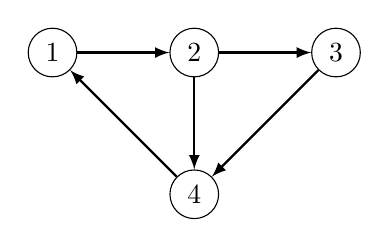
\begin{tikzpicture}[scale=0.9]
\node[draw, circle] (1) at (1,3) {$1$};
\node[draw, circle] (2) at (3,3) {$2$};
\node[draw, circle] (3) at (5,3) {$3$};
\node[draw, circle] (4) at (3,1) {$4$};

\path[draw,thick,->,>=latex] (1) -- (2);
\path[draw,thick,->,>=latex] (2) -- (3);
\path[draw,thick,->,>=latex] (2) -- (4);
\path[draw,thick,->,>=latex] (3) -- (4);
\path[draw,thick,->,>=latex] (4) -- (1);
\end{tikzpicture}
\end{center}
これは隣接リストで次のように表現できます。
\begin{lstlisting}
adj[1].push_back(2);
adj[2].push_back(3);
adj[2].push_back(4);
adj[3].push_back(4);
adj[4].push_back(1);
\end{lstlisting}

グラフが無向の場合は両方から互いに対して辺を張ることで表現できます。

重み付きグラフの場合は少し持たせ方を変えます。

\begin{lstlisting}
vector<pair<int,int>> adj[N];
\end{lstlisting}


このとき、ノード$a$の隣接リストには、ノード$a$からノード$b$へ重み$w$の辺
があるとき、$(b, w)$のpairを作ります。
例えば、次の例を考えます。

\begin{center}
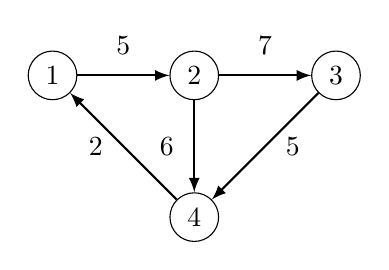
\begin{tikzpicture}[scale=0.9]
\node[draw, circle] (1) at (1,3) {$1$};
\node[draw, circle] (2) at (3,3) {$2$};
\node[draw, circle] (3) at (5,3) {$3$};
\node[draw, circle] (4) at (3,1) {$4$};

\path[draw,thick,->,>=latex] (1) -- node[font=\small,label=above:5] {} (2);
\path[draw,thick,->,>=latex] (2) -- node[font=\small,label=above:7] {} (3);
\path[draw,thick,->,>=latex] (2) -- node[font=\small,label=left:6] {} (4);
\path[draw,thick,->,>=latex] (3) -- node[font=\small,label=right:5] {} (4);
\path[draw,thick,->,>=latex] (4) -- node[font=\small,label=left:2] {} (1);
\end{tikzpicture}
\end{center}
これは次のように表現できます。
\begin{lstlisting}
adj[1].push_back({2,5});
adj[2].push_back({3,7});
adj[2].push_back({4,6});
adj[3].push_back({4,5});
adj[4].push_back({1,2});
\end{lstlisting}


隣接リストを用いる利点は、
あるノードから辺を経由して移動できるノードを効率的に見つけられることです。
例えば、以下のfor文で、ノード$s$から移動できるすべてのノードを処理できます。

\begin{lstlisting}
for (auto u : adj[s]) {
    // process node u
}
\end{lstlisting}

\subsubsection{隣接行列形式 - Adjacency matrix representation}

\index{adjacency matrix}

\key{隣接行列}は、
辺を2次元の配列で表現します。
2つのノード間にエッジがあるかどうかを効率的に調べることができます。
\begin{lstlisting}
int adj[N][N];
\end{lstlisting}
ここで、$\texttt{adj}[a][b]$ は、グラフにノード $a$ からノード $b$ への辺が含まれるかをしめし、
$\texttt{adj}[a][b]=1$なら辺があることを、
$\texttt{adj}[a][b]=0$なら辺がないことを示します。

例えば次のグラフを考えます。
\begin{center}
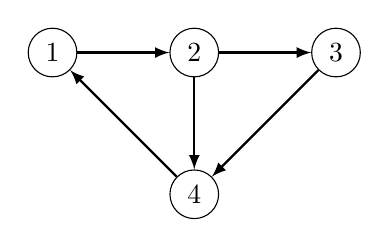
\begin{tikzpicture}[scale=0.9]
\node[draw, circle] (1) at (1,3) {$1$};
\node[draw, circle] (2) at (3,3) {$2$};
\node[draw, circle] (3) at (5,3) {$3$};
\node[draw, circle] (4) at (3,1) {$4$};

\path[draw,thick,->,>=latex] (1) -- (2);
\path[draw,thick,->,>=latex] (2) -- (3);
\path[draw,thick,->,>=latex] (2) -- (4);
\path[draw,thick,->,>=latex] (3) -- (4);
\path[draw,thick,->,>=latex] (4) -- (1);
\end{tikzpicture}
\end{center}
次のように示せます。
\begin{center}
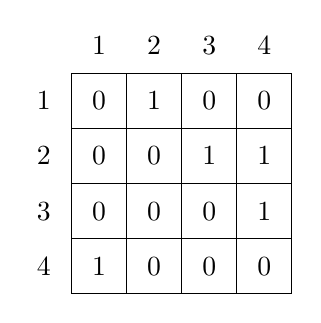
\begin{tikzpicture}[scale=0.7]
\draw (0,0) grid (4,4);
\node at (0.5,0.5) {1};
\node at (1.5,0.5) {0};
\node at (2.5,0.5) {0};
\node at (3.5,0.5) {0};
\node at (0.5,1.5) {0};
\node at (1.5,1.5) {0};
\node at (2.5,1.5) {0};
\node at (3.5,1.5) {1};
\node at (0.5,2.5) {0};
\node at (1.5,2.5) {0};
\node at (2.5,2.5) {1};
\node at (3.5,2.5) {1};
\node at (0.5,3.5) {0};
\node at (1.5,3.5) {1};
\node at (2.5,3.5) {0};
\node at (3.5,3.5) {0};
\node at (-0.5,0.5) {4};
\node at (-0.5,1.5) {3};
\node at (-0.5,2.5) {2};
\node at (-0.5,3.5) {1};
\node at (0.5,4.5) {1};
\node at (1.5,4.5) {2};
\node at (2.5,4.5) {3};
\node at (3.5,4.5) {4};
\end{tikzpicture}
\end{center}

辺に重みがある場合は隣接行列の表現を拡張します。
$adj[a][b]$の値としてエッジの重みが含まれるようにします。
例を示します。

\begin{center}
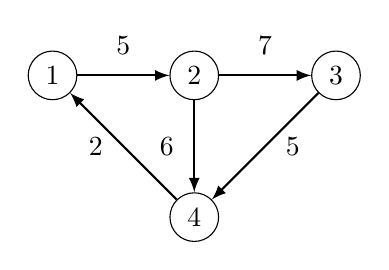
\begin{tikzpicture}[scale=0.9]
\node[draw, circle] (1) at (1,3) {$1$};
\node[draw, circle] (2) at (3,3) {$2$};
\node[draw, circle] (3) at (5,3) {$3$};
\node[draw, circle] (4) at (3,1) {$4$};

\path[draw,thick,->,>=latex] (1) -- node[font=\small,label=above:5] {} (2);
\path[draw,thick,->,>=latex] (2) -- node[font=\small,label=above:7] {} (3);
\path[draw,thick,->,>=latex] (2) -- node[font=\small,label=left:6] {} (4);
\path[draw,thick,->,>=latex] (3) -- node[font=\small,label=right:5] {} (4);
\path[draw,thick,->,>=latex] (4) -- node[font=\small,label=left:2] {} (1);
\end{tikzpicture}
\end{center}
\begin{samepage}
これは次のように表現できます。
\begin{center}
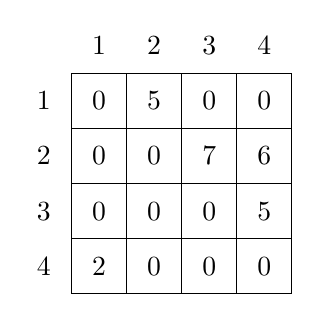
\begin{tikzpicture}[scale=0.7]
\draw (0,0) grid (4,4);
\node at (0.5,0.5) {2};
\node at (1.5,0.5) {0};
\node at (2.5,0.5) {0};
\node at (3.5,0.5) {0};
\node at (0.5,1.5) {0};
\node at (1.5,1.5) {0};
\node at (2.5,1.5) {0};
\node at (3.5,1.5) {5};
\node at (0.5,2.5) {0};
\node at (1.5,2.5) {0};
\node at (2.5,2.5) {7};
\node at (3.5,2.5) {6};
\node at (0.5,3.5) {0};
\node at (1.5,3.5) {5};
\node at (2.5,3.5) {0};
\node at (3.5,3.5) {0};
\node at (-0.5,0.5) {4};
\node at (-0.5,1.5) {3};
\node at (-0.5,2.5) {2};
\node at (-0.5,3.5) {1};
\node at (0.5,4.5) {1};
\node at (1.5,4.5) {2};
\node at (2.5,4.5) {3};
\node at (3.5,4.5) {4};
\end{tikzpicture}
\end{center}
\end{samepage}

隣接行列表現の欠点として行列が$n^2$要素分のメモリを必要とし、
通常はそのほとんどが$0$となってしまうためです。
このため、グラフが大きい場合はこの表現は適しません。

\subsubsection{エッジリスト形式 - Edge list representation}

\index{edge list}

\key{エッジリスト}形式は、全ての辺を順序通りに保管したものです。
アルゴリズムがグラフのすべてのエッジを処理する必要に便利です。
ただし、あるノードから始まるエッジを見つける必要がない場合は適しません。

次のように情報を持たせます。
\begin{lstlisting}
vector<pair<int,int>> edges;
\end{lstlisting}
$(a,b)$ に辺があることを示します。
例を示します。

\begin{center}
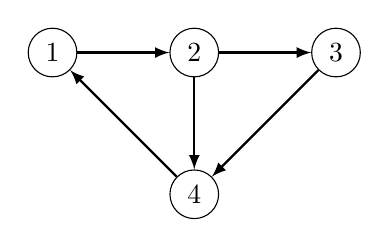
\begin{tikzpicture}[scale=0.9]
\node[draw, circle] (1) at (1,3) {$1$};
\node[draw, circle] (2) at (3,3) {$2$};
\node[draw, circle] (3) at (5,3) {$3$};
\node[draw, circle] (4) at (3,1) {$4$};

\path[draw,thick,->,>=latex] (1) -- (2);
\path[draw,thick,->,>=latex] (2) -- (3);
\path[draw,thick,->,>=latex] (2) -- (4);
\path[draw,thick,->,>=latex] (3) -- (4);
\path[draw,thick,->,>=latex] (4) -- (1);
\end{tikzpicture}
\end{center}
これは次のように表現できます。
\begin{lstlisting}
edges.push_back({1,2});
edges.push_back({2,3});
edges.push_back({2,4});
edges.push_back({3,4});
edges.push_back({4,1});
\end{lstlisting}

\noindent
グラフに重みがある場合、以下のように持たせることができます。
\begin{lstlisting}
vector<tuple<int,int,int>> edges;
\end{lstlisting}
各要素は$(a, b, w)$であり、ノード$a$からノード$b$へ重み$w$の辺があることを意味します。
例を示します。

\begin{center}
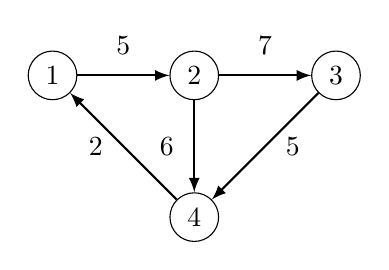
\begin{tikzpicture}[scale=0.9]
\node[draw, circle] (1) at (1,3) {$1$};
\node[draw, circle] (2) at (3,3) {$2$};
\node[draw, circle] (3) at (5,3) {$3$};
\node[draw, circle] (4) at (3,1) {$4$};

\path[draw,thick,->,>=latex] (1) -- node[font=\small,label=above:5] {} (2);
\path[draw,thick,->,>=latex] (2) -- node[font=\small,label=above:7] {} (3);
\path[draw,thick,->,>=latex] (2) -- node[font=\small,label=left:6] {} (4);
\path[draw,thick,->,>=latex] (3) -- node[font=\small,label=right:5] {} (4);
\path[draw,thick,->,>=latex] (4) -- node[font=\small,label=left:2] {} (1);
\end{tikzpicture}
\end{center}
\begin{samepage}
これは次のように表現できます。\footnote{In some older compilers, the function
\texttt{make\_tuple} must be used instead of the braces (for example,
\texttt{make\_tuple(1,2,5)} instead of \texttt{\{1,2,5\}}).}:
\begin{lstlisting}
edges.push_back({1,2,5});
edges.push_back({2,3,7});
edges.push_back({2,4,6});
edges.push_back({3,4,5});
edges.push_back({4,1,2});
\end{lstlisting}
\end{samepage}
